% MXR4DOT -- VLSID 2027. 6 pages incl. references, IEEE two-column, double-blind.
\documentclass[conference]{IEEEtran}

\newif\ifanon      \anontrue
\newif\ifdraft     \drafttrue

\usepackage{cite}
\usepackage{amsmath,amssymb,amsfonts}
\usepackage{algorithmic}
\usepackage{graphicx}
\usepackage{tikz}
\usetikzlibrary{positioning,calc,arrows.meta,decorations.pathreplacing,fit,shapes.geometric}
\usepackage{textcomp}
\usepackage{xcolor}
\usepackage{booktabs}
\usepackage{colortbl}
\usepackage{multirow}
\usepackage{siunitx}
\usepackage[caption=false,font=footnotesize]{subfig}
\usepackage{balance}
\usepackage[hidelinks]{hyperref}

\graphicspath{{figures/}}

\sisetup{detect-weight=true, detect-family=true, group-separator={,},
  range-phrase={--}, range-units=single, per-mode=symbol}
\DeclareSIUnit{\flop}{FLOP}

\ifdraft
  \newcommand{\TODO}[1]{\textcolor{red}{\textbf{[TODO: #1]}}}
  \newcommand{\DATAGAP}[1]{\textcolor{blue}{\textbf{[DATA: #1]}}}
\else
  \newcommand{\TODO}[1]{}
  \newcommand{\DATAGAP}[1]{}
\fi

\newcommand{\projname}{\textsc{MxR4Dot}}
\newcommand{\fpfour}{MXFP4}
\newcommand{\fpeight}{MXFP8}
\newcommand{\fpfourres}{MXFP4R}
\newcommand{\mtwo}{M\textsuperscript{2}XFP4}
\newcommand{\xif}{CV-X-IF}
\newcommand{\core}{CV32E40X}
\newcommand{\anchor}{\alpha}

\newcommand{\insn}[1]{\texttt{\small #1}}
\newcommand{\MXFUSED}{\insn{mxfused}}
\newcommand{\MXDOTP}{\insn{mxr4dot}}
\newcommand{\MXFINAL}{\insn{mxfinal}}

\begin{document}

\title{\projname: A Residue MX Format in a RISC-V Coprocessor for Evaluating
  Hardware Cost Against Existing MX Formats \TODO{working title}}

\ifanon
  \author{\IEEEauthorblockN{Anonymous Submission}
          \IEEEauthorblockA{Paper ID: \TODO{SoftConf}}}
\else
  \author{\IEEEauthorblockN{Author One, Author Two}
          \IEEEauthorblockA{Affiliation}}
\fi

\maketitle

\begin{abstract}
Four-bit Microscaling (MX) formats reach acceptable accuracy for many
inference workloads, but some models and deployment targets demand more
precision than a single four-bit block provides, without conceding the memory
advantage that motivates four-bit weights in the first place. Several augmented
MX variants address this at the format level; their hardware cost, however, is
seldom measured against the alternatives they displace on common silicon.

This work introduces \fpfourres, an MX variant that represents activations as
the sum of two \fpfour{} blocks under independent block scales while keeping
weights in plain \fpfour, and evaluates whether it merits a hardware
implementation. Because only activations carry the second block, weight
footprint remains that of \fpfour{} while representational precision approaches
that of \fpeight. The value of this trade depends on delivered throughput,
which a format-level analysis cannot establish.

We implement \fpfourres{} alongside \fpfour, \fpeight, and \mtwo{} as
format-specialised independent dot-product engines within a single \xif-compliant
coprocessor (CV32E40X), characterising all four on one host core, one synthesis flow, and
one technology node. Each engine accumulates in a scale-free frame whose width
depends on the element format alone.

Synthesised at \SI{45}{\nano\meter}, the specialised \fpfour{} engine sustains
\SI{5.1}{\times} the throughput per unit area of \fpeight. The \fpfourres{}
datapath requires three source operands and two block scales, exceeding a
three-read-port register file, and is expressed as an instruction pair whose
present throughput is \DATAGAP{X}$\times$ that of \fpeight; its advantage
therefore lies in halved weight memory at comparable accuracy rather than in
compute.
\end{abstract}


\begin{IEEEkeywords}
Microscaling formats, MXFP8, RISC-V, CV-X-IF, dot product, low-precision
arithmetic, ASIC synthesis.
\end{IEEEkeywords}

\section{Introduction}
\label{sec:intro}

Microscaling (MX) formats, standardised by the Open Compute
Project~\cite{ocp2023mx}, associate a block of $k$ elements with one 8-bit
power-of-two exponent (E8M0) and encode each element in a narrow floating-point
type. Four-bit MX has been shown adequate for a range of inference and even
training workloads~\cite{rouhani2023microscaling}, yet its single shared
power-of-two scale bounds the precision available within a block. Workloads
sensitive to this bound have motivated augmented four-bit formats:
\mtwo{}~\cite{m2xfp2026} allocates per-subgroup metadata to recover precision,
and NVFP4 format replaces the conventional E8M0 block scale with a higher-precision FP8 block scale. These are proposed
and evaluated as data formats; their realisation cost, measured against the formats they would replace on identical hardware, is largely absent from the
literature.

This work examines a further variant that we propose, \fpfourres, in which an activation block
is represented as the sum of two \fpfour{} blocks carrying independent E8M0
scales, while weight blocks remain plain \fpfour. The construction is
asymmetric by design: weight footprint is that of \fpfour, whereas activation
precision approaches that of \fpeight. For inference, where weights dominate
memory and bandwidth, this is a favourable position \emph{if} the arithmetic
can be executed at competitive throughput.

That condition is the subject of the paper. A \fpfourres{} dot product forms
two product terms under two independent scales and therefore needs three
genuine 64-bit vector operands and two independent block scales at once,
exceeding a three-read-port register file. The resulting throughput cannot be
inferred from the format definition and must be measured on synthesised
hardware. We do so by implementing \fpfourres{} together with \fpfour,
\fpeight, and \mtwo{} as independent, format-specialised engines behind one
coprocessor, and
characterising all four on a common core, synthesis flow, and technology node.

\subsection{Related work}
\label{sec:intro-related}

Two RISC-V extensions for MX dot products precede this
work. MXDOTP~\cite{islamoglu2025mxdotp} adds an \fpeight{} dot-product unit to
a Snitch core and supplies block scales through Stream Semantic Registers.
VMXDOTP~\cite{wipfli2026vmxdotp} extends the RISC-V Vector specification to
cover \fpeight{} and \fpfour, resolving operand-port pressure by
time-multiplexing vector register-file reads, and reports
\SI{250}{\giga\flop\per\second} at \SI{1632}{\giga\flop\per\second\per\watt}
for \fpfour{} in \SI{12}{\nano\meter}. This work targets a different point in
the design space: a coprocessor behind the standardised \xif{} interface,
hosted by a compact embedded core, covering formats these extensions do not.
Neither prior extension supports \mtwo{} nor our proposed \fpfourres.

The accumulation datapath common to all three works derives from the anchored
fixed-point scheme of Lutz \emph{et al.}~\cite{lutz2024fp8dot}, which
MXDOTP extended to the two independent block scales of an MX dot product. The
present contribution is the derivation of this scheme for four distinct
formats, each with its own frame geometry.

\mtwo{} was introduced as an algorithm–hardware co-design with a systolic-array
accelerator~\cite{m2xfp2026}; the engine described here is a RISC-V coprocessor
realisation that re-derives the per-subgroup top-1 element within the datapath.

\subsection{Contributions}
\label{sec:intro-contrib}

\begin{enumerate}
  \item \fpfourres, a residue MX format, and its hardware evaluation: on a
        common \SI{45}{\nano\meter} flow, its throughput relative to \fpeight{}
        is \DATAGAP{X}$\times$ (\S\ref{sec:eval-residue}), locating its benefit
        in weight memory (\S\ref{sec:analysis}) rather than compute.
  \item A four-format comparison of \fpfour, \fpeight, \mtwo, and \fpfourres{}
        on one host core and one synthesis flow, removing the process and
        system-scope differences that complicate cross-paper MX comparisons
        (\S\ref{sec:eval}).
  \item A per-format scale-free accumulation frame, with anchor and width
        derived in closed form for each format and shown tight against exact
        rational arithmetic over the full E8M0 scale range
        (\S\ref{sec:arch-frame}).
  \item A coprocessor conforming to the \xif{} interface, portable across
        compliant host cores (\S\ref{sec:bg-xif}).
\end{enumerate}
\section{Background}
\label{sec:background}

\subsection{Microscaling formats}
\label{sec:bg-mx}

An MX block comprises $k$ elements sharing a single E8M0 scale
$2^{S-127}$, $S \in [0,254]$. The OCP specification fixes $k=32$; the
architectural granularity in this design is the 16-element half-block carried
by a 64-bit dual-read operand pair. Elements are E2M1 for \fpfour{} and E4M3 or
E5M2 for \fpeight. For two blocks $A$, $B$ with scales $s_a=2^{S_a-127}$,
$s_b=2^{S_b-127}$ accumulating into an FP32 value, the scaled dot product is
%
\begin{equation}
  \label{eq:base}
  \mathit{acc}' = s_a s_b \sum_i a_i b_i + \mathit{acc}.
\end{equation}
%
Both scales are powers of two, so applying them is an exponent adjustment
rather than a multiplication. Rewriting~\eqref{eq:base} to expose this,
%
\begin{equation}
  \label{eq:factor}
  \mathit{acc}' = s_a s_b\!\left( \sum_i a_i b_i
                  + \frac{\mathit{acc}}{s_a s_b} \right),
\end{equation}
%
places the products at a fixed fixed-point position and admits the accumulator
by a shift of $E_{\mathit{acc}} - \mathrm{bias} - (S_a{+}S_b{-}254)$ bit
positions, where $E_{\mathit{acc}}$ is the accumulator's biased exponent. No
multiplier is required on the datapath; the block scale reappears only in the
final exponent. Equation~\eqref{eq:factor} is the identity every engine
realises.

\subsection{Coprocessor interface}
\label{sec:bg-xif}

The host core, \core, is designed within OpenHW Group's CORE-V family to
extend the ISA through an external coprocessor over \xif{} rather than by
embedding custom functional units in its own pipeline, which keeps the
coprocessor's cost isolated and measurable rather than conflated with changes
to the host itself. The coprocessor attaches over \xif~\cite{openhw_cvxif} and
uses only the standardised issue, commit, and result channels, with no private
path into the host pipeline; any XIF compliant core supporting three source
reads and dual-read can host it. The host in this work, \core, does not
implement \xif's optional dual-read, which was added to its register-file read
path; the modification is independent of the coprocessor, which uses only the
standard interface.

\subsection{Motivation for \fpfourres}
\label{sec:bg-motiv}

\fpfour{} halves weight footprint versus \fpeight{} but at a real cost in accuracy~\cite{m2xfp2026}; uniform \fpeight{} recovers that accuracy but surrenders the memory-bandwidth advantage and widens the accumulation datapath. Asymmetric precision offers a middle path. On GPT-2/WikiText-2, naive \fpfour{} collapses perplexity from 30.3 to 107.8; adding a second \fpfour{} block to activations alone (\fpfourres, averaging 6.375\,b/element) recovers \SI{93}{\percent} of that loss, against \SI{36}{\percent} for the mirrored weight-side allocation. This activation-side advantage is not universal, however: \S\ref{sec:analysis} shows where it holds, where it inverts, and why.
\section{\fpfourres{} Analysis}
\label{sec:analysis}

Whether \fpfourres{} merits implementation depends on its post-training accuracy across model types. Table~\ref{tab:accuracy} reports the four implemented formats, NVFP4, and two single-sided ablations across nine models in three modalities.

\textbf{Quantisation Protocol.} Quantisation is post-training and calibration-free: weights use static per-block scaling ($k=32$, OCP), activations use dynamic scaling from each tensor's peak magnitude, and all formats round to nearest-even. Language model evaluations average two seeds; vision and speech use a single seed (Table~\ref{tab:accuracy}, footnote).

\begin{table*}[t]
  \centering
  \caption{Post-training quantisation accuracy. WikiText-2 perplexity
           ($\downarrow$), ImageNet-1k top-1 ($\uparrow$), LibriSpeech
           test-clean WER ($\downarrow$). All layers quantised; BF16 is the
           unquantised reference. The two rules below \fpfourres{} are
           single-sided and symmetric ablations of the residue construction.}
  \label{tab:accuracy}
  \setlength{\tabcolsep}{4pt}
  \renewcommand{\arraystretch}{1.1}
  \small
  \begin{tabular}{|l|r|r|r|r|r|r|r|}
    \hline
    & \multicolumn{4}{c|}{Perplexity $\downarrow$}
    & \multicolumn{2}{c|}{Top-1 $\uparrow$}
    & WER $\downarrow$ \\
    \hline
    Format & GPT-2 & Llama-2 & Llama-3 & Mistral & ViT-B\textdagger & RN-50\textdagger & wav2vec2\textdagger \\
           &       & 7\,B    & 8\,B    & 7\,B    &       &       &          \\
    \hline
    BF16   & 30.3 & 6.02 & 6.74 & 6.14 & 80.3 & 80.4 & 2.86 \\
    \hline
    \fpfour             & 107.8 & 7.83 & 9.19 & 7.90 & 73.6 & 11.3 & 9.00 \\
    \hline
    NVFP4               &  36.3 & \underline{6.38} & \underline{7.59} & 6.46 & 77.3 & 55.5 & \underline{3.68} \\
    \hline
    \mtwo               &  46.4 & 6.46 & 7.85 & \underline{6.35} & \underline{78.4} & 60.3 & 5.00 \\
    \hline
    \rowcolor{gray!12}
    \textbf{\fpfourres{} (residue on A)} & \textbf{\underline{35.4}} & \textbf{6.65} & \textbf{7.75} & \textbf{6.49} & \textbf{78.1} & \textbf{27.2} & \textbf{30.5} \\
    \hline
    \quad \textbf{\textit{residue on W}}    & \textbf{79.7} & \textbf{6.73} & \textbf{7.82} & \textbf{6.77} & \textbf{77.2} & \textbf{\underline{67.3}} & \textbf{4.27} \\
    \hline
    \quad \textit{residue on both} &  30.3 & 6.04 & 6.79 & 6.15 & 80.3 & 79.3 & 2.77 \\
    \hline
    \fpeight-E4M3       &  31.1 & 6.08 & 6.87 & 6.20 & 79.5 & 77.9 & 2.71 \\
    \hline
  \end{tabular}
  \\[2pt]
  \begin{minipage}{\textwidth}
    \footnotesize
    \underline{Underline}: best among MXFP4 / NVFP4 / \mtwo{} / \fpfourres{} (residue on A) per column (BF16 and \fpeight-E4M3 are reference points, not candidates).
    \fpfourres{} (default) places residue on activations only (W/A $=4.25/8.50$\,b); ``residue on W'' is mirrored ($8.50/4.25$\,b) and ``residue on both'' is symmetric ($8.50/8.50$\,b).
    \textdagger vision/speech: single seed (42).
  \end{minipage}
\end{table*}

Symmetric residue matches BF16 and \fpeight{} accuracy everywhere, confirming that two independent \fpfour{} blocks are an adequate substitute for one \fpeight{} block. Restricting the residue to activations alone, however, is not universally optimal: it recovers most of the accuracy gap on seven of nine evaluated models, including GPT-2, all three larger language models, and the vision transformer, but the preference inverts on the deeper convolutional network and the speech model, where naive \fpfour{} already collapses badly and weight-side residue instead dominates recovery. The inversion is not explained by architecture family or parameter volume: two closely related convolutional networks land on opposite sides despite near-identical weight-to-activation ratios. A per-layer error diagnostic offers real mechanistic insight (below), though it explains why an allocation fails more reliably than it predicts which allocation will win.

For the speech model, neither candidate explanation holds up: a sign-correlation test rules out error cancellation between weight and activation terms, and the error is not concentrated in the audio front end. The actual mechanism is subtler: activation-side residue collapses a large but symmetric, self-averaging quantisation error at one late, decoder-critical layer, but in doing so leaves a smaller, systematic per-channel weight bias as the dominant remaining error there instead. That structured bias proves more damaging to sequence decoding than the larger, unstructured noise it replaces. The result generalises beyond this format: reducing reconstruction error is not always sufficient when the reduction changes the character of the error, not just its size, at a decision-critical layer.

\fpfourres{} offers two single-sided configurations, placing the residue block on activations or on weights, and their strengths fall on different workloads. The activation-side variant achieves the lowest perplexity among all four-bit candidates on the compact decoder (GPT-2) and outperforms \mtwo{} on Llama-3-8B, though NVFP4 leads on the larger language models overall. The weight-side variant wins outright on the deeper convolutional network and outperforms \mtwo{} on the speech model. The two formats are therefore complementary rather than competing, motivating exposing both as independent coprocessor engines (\S\ref{sec:arch-engines}).

\subsection{Zero-shot task validation}
\label{sec:analysis-zeroshot}

\begin{table}[t]
  \centering
  \caption{Zero-shot task accuracy (\SI{}{\percent}) on downstream benchmark evaluations for GPT-2 and Llama-2-7B. Bold indicates the higher-performing single-sided residue allocation.}
  \label{tab:zeroshot}
  \setlength{\tabcolsep}{2.5pt}
  \renewcommand{\arraystretch}{1.1}
  \scriptsize
  \begin{tabular}{|l|l|r|r|r|r|r|}
    \hline
    Model & Task & BF16 & \fpfour & \mtwo & \fpfourres{} (Act) & \fpfourres{} (Wt) \\
    \hline
    GPT-2 & WinoGrande & 51.6 & 48.5 & 49.8 & \textbf{52.6} & 51.7 \\
    \hline
          & PIQA       & 62.3 & 58.2 & 60.1 & \textbf{61.4} & 58.3 \\
    \hline
          & HellaSwag  & 31.3 & 29.0 & 30.6 & \textbf{29.9} & 29.8 \\
    \hline
          & ARC-Easy   & 40.2 & 38.3 & 37.8 & \textbf{39.5} & 38.7 \\
    \hline
          & BoolQ\textdagger & 50.2 & 59.6 & 57.6 & 57.6 & 56.7 \\
    \hline
    Llama-2-7B & WinoGrande & 69.1 & 66.5 & 67.6 & \textbf{68.8} & 68.1 \\
    \hline
               & PIQA       & 78.4 & 76.9 & 77.8 & \textbf{77.9} & 77.5 \\
    \hline
               & HellaSwag  & 76.1 & 70.6 & 74.5 & \textbf{74.1} & 74.0 \\
    \hline
               & ARC-Easy   & 74.1 & 69.4 & 73.4 & \textbf{72.3} & 71.3 \\
    \hline
               & BoolQ      & 79.4 & 72.8 & 77.3 & \textbf{77.1} & 76.6 \\
    \hline
  \end{tabular}
  \\[2pt]
  \begin{minipage}{\columnwidth}
    \footnotesize
    \textdagger GPT-2 unquantised (BF16) accuracy on BoolQ is statistically indistinguishable from the \SI{50}{\percent} chance baseline; nominal gains under quantisation represent noise and are excluded from average gap recovery calculations.
  \end{minipage}
\end{table}


Five zero-shot reasoning benchmarks (Table~\ref{tab:zeroshot}) corroborate the perplexity-level findings: activation-side residue outperforms weight-side residue on four of five tasks for both the compact decoder and the instruction-tuned model, recovering \SI{78}{\percent} and \SI{67}{\percent} of the quantisation gap respectively (the compact decoder's near-chance BoolQ baseline excluded). \mtwo{} follows the same ordering under zero-shot evaluation as under perplexity, trailing activation-only residue on the compact decoder but competitive on the instruction-tuned model.
\section{Microarchitecture}
\label{sec:arch}

\subsection{Residue and metadata-augmented variants}
\label{sec:arch-variants}

\fpfourres{} adds a second activation block $\mathit{ar}$ with its own scale
$s_{ar}=2^{S_{ar}-127}$, quantising the residual of the primary block against
plain \fpfour{} weights. The dot product carries two independent scales,
%
\begin{equation}
  \label{eq:res-base}
  \mathit{acc}' = s_a s_w \sum_i a_i w_i
                + s_{ar} s_w \sum_i \mathit{ar}_i w_i + \mathit{acc},
\end{equation}
%
which factors on the primary scale as
%
\begin{equation}
  \label{eq:res-factor}
  \mathit{acc}' = s_a s_w\!\left( \sum_i a_i w_i
                  + \frac{s_{ar}}{s_a} \sum_i \mathit{ar}_i w_i
                  + \frac{\mathit{acc}}{s_a s_w} \right).
\end{equation}
%
The ratio $s_{ar}/s_a = 2^{S_{ar}-S_a}$ is again a shift, by
$\delta = S_a - S_{ar} \ge 0$; \S\ref{sec:arch-residue} establishes the
non-negativity and its role in placement. The primary product term reuses the
\fpfour{} datapath unchanged.

\mtwo{}~\cite{m2xfp2026} retains E2M1 elements and adds per-instruction
metadata. Within each 8-element subgroup, two bits extend the largest-magnitude
activation element to E2M3, and two bits refine the weight subgroup scale to
$(1+\kappa/4)\,2^{S}$, $\kappa\in\{0,1,2,3\}$. The scaled sum of products
becomes
%
\begin{equation}
  \label{eq:m2}
  \mathit{acc}' = s_a s_w \sum_g \left(1+\tfrac{\kappa_g}{4}\right)
                  \sum_{i \in g} a_i w_i + \mathit{acc},
\end{equation}
%
in which $a_i$ denotes the top-1 element's E2M3-corrected value for the
subgroup's single largest-magnitude activation and its plain E2M1 value
otherwise, and the $\kappa_g$ factor is a per-subgroup shift-and-add on the
partial sum, not a multiplication.

\subsection{Instruction interface}
\label{sec:arch-isa}

Instructions reuse the R4-type FMADD.S operand layout, so a third source needs
no host register-file change.

% Merged instruction set + operand map. R4-type custom-0 opcode 0x0B; funct2
% selects the MX format, funct3 the operation. Only MXFP4R takes two native
% instructions (stated in the caption; no separate Insns/dp column needed).
% Column headers abbreviated (f3/f2, Elems) with symbol-footnote expansions
% to fit the operand columns in the same single-column float; symbol
% definitions and dual-read/32-bit-read facts follow below.
\begin{table}[t]
  \centering
  \caption{Instruction set and operand map. R4-type, custom-0 opcode
           \insn{0x0B}; \insn{funct2} selects the MX format, \insn{funct3}
           the operation. \fpfourres{} requires two native instructions,
           since it carries a third \SI{64}{\bit} source
           and a second block scale (\S\ref{sec:arch-residue}).}
  \label{tab:isa}
  \scriptsize
  \setlength{\tabcolsep}{2.3pt}
  \renewcommand{\arraystretch}{1.15}
  \resizebox{\columnwidth}{!}{%
  \begin{tabular}{|l|l|c|c|c|c|c|}
    \hline
    Format & Mnemonic & \insn{f3/f2}\rlap{$^{\ast}$} &
      Elems\rlap{$^{\dagger}$} &
      \insn{rs1} & \insn{rs2} & \insn{rs3} \\
    \hline
    \fpfour  & \MXFUSED & 011/00 & 16
        & $p_A$ & $p_W$ & $\{x_W,x_A,\mathit{acc}\}$ \\
    \hline
    \fpeight & \MXFUSED & 011/11 &  8
        & $p_A$ & $p_W$ & $\{x_W,x_A,\mathit{acc}\}$ \\
    \hline
    \mtwo    & \MXFUSED & 011/10 & 16
        & $p_A$ & $p_W$ & $\{\mathrm{md},x_W,x_A,\mathit{acc}\}$ \\
    \hline
    \multirow{2}{*}{\fpfourres}
             & \MXDOTP  & 000/01 & 16
                 & $p_A$ & $p_W$ & $p_{Ar}$ \\
    \cline{2-7}
             & \MXFINAL & 001/01 & ---
                 & $\{x_A,x_{Ar},x_W\}$ & $\mathit{acc}$ & --- \\
    \hline
  \end{tabular}%
  }
  \\[2pt]
  \begin{minipage}{\columnwidth}
    \scriptsize
    \textsuperscript{*}\insn{funct3}/\insn{funct2}.
    \textsuperscript{\textdagger}Elements per instruction.
    $p_A,p_W,p_{Ar}$: packed activation/weight/residue-activation vectors;
    $x_A,x_{Ar},x_W$: E8M0 block scales; \textit{acc}: FP32 accumulator;
    braces denote fields packed into one register word. $p_A,p_W,p_{Ar}$ and
    \MXFUSED's \insn{rs3} are \SI{64}{\bit} dual-read register pairs;
    \MXFINAL's \insn{rs1},\insn{rs2} are plain \SI{32}{\bit} reads.
    \MXDOTP{} writes no register; \MXFINAL{} and \MXFUSED{} write the FP32
    result.
  \end{minipage}
\end{table}

\MXFUSED{} is a single-instruction operation for \fpfour, \fpeight, and \mtwo.
\fpfourres{} instead needs three genuine 64-bit sources and two independent
block scales at once, which exceeds a three-read-port register file, so it is
issued as the \MXDOTP/\MXFINAL{} pair (\S\ref{sec:arch-residue}). For \mtwo{},
operand order is significant: \insn{rs1} carries activations and \insn{rs2}
weights.

\subsection{Scale-free accumulation frame}
\label{sec:arch-frame}

Every engine realises~\eqref{eq:factor} through a fixed-point frame in which
the sum of products is resident and the accumulator, rather than the products,
absorbs the block scale~\cite{lutz2024fp8dot,islamoglu2025mxdotp}. The sum of
products occupies a format-specific anchor position, where frame bit $b$ carries
weight $2^{b-\alpha}$ and the anchor $\alpha$ is chosen so that the smallest
representable quantum aligns with bit~0; every product is then frame-resident
without a shifter. The anchor thus tracks each format's smallest quantum:
$\alpha=2$ for \fpfour's E2M1 products, $32$ for \fpeight, whose smallest E5M2
subnormal product is $2^{-32}$,\footnote{The reference
implementation~\cite{islamoglu2025mxdotp} anchors at $34$; its per-element decode
pads the E5M2 mantissa by one bit, shifting the same 95-bit frame up two
positions, so the two are value-identical.} and $6$ for \mtwo, set by the $1/64$
quantum its $(1+\kappa/4)$ refinement introduces; \fpfourres{} shares \fpfour's
anchor. The FP32 accumulator enters by a shift of
$E_{\mathit{acc}} - C_\alpha - (S_a{+}S_b{-}254)$, where $C_\alpha = 150-\alpha$
is a compile-time constant, and bits below the frame are retained in a
$\mathrm{REMAIN}$-bit extension with a sticky bit. The scale contributes only to
the final exponent.

The consequence is that frame width is a function of the element format alone
and is independent of the E8M0 scale range, so each engine is exact to
round-to-nearest-even over every legal scale pair and every FP32 accumulator at
a width set by its own format. Applying the scheme across four formats requires
a distinct frame geometry for each; the constants are derived in closed form and
listed in Table~\ref{tab:frames}.

\begin{table}[t]
  \centering
  \caption{Derived sliding-frame constants. Frame width is set by the element
           format alone; the E8M0 scale range does not appear.}
  \label{tab:frames}
  \setlength{\tabcolsep}{4pt}
  \renewcommand{\arraystretch}{1.15}
  \begin{tabular}{|l|c|c|c|c|c|}
    \hline
    Engine & Anchor $\anchor$ & $\Sigma_{\mathrm{P}}$\rlap{$^{\ast}$} & Frame & REMAIN & LZC \\
           &                  & (bits)                & (bits) & (bits) & (bits) \\
    \hline
    \fpfour     &  2 & 12 & 38 & 25 &  63 \\
    \hline
    \fpeight    & 32 & 69 & 95 & 25 & 120 \\
    \hline
    \mtwo       &  6 & 17 & 43 & 25 &  68 \\
    \hline
    \fpfourres  &  2 & 12\rlap{$^{\dagger}$} & 38 & 36 &  74 \\
    \hline
  \end{tabular}
  \\[2pt]
  \begin{minipage}{\columnwidth}
    \footnotesize
    $^{\ast}$Unsigned sum-of-products field resident in the frame word.
    $^{\dagger}$Two product terms at independent scales
    (\S\ref{sec:arch-residue}); the wider REMAIN follows from cancellation
    between them rather than against the accumulator.
  \end{minipage}
\end{table}

Three of the table's columns are linked as consistency checks: Frame $=
26+\Sigma_{\mathrm{P}}$ (sign, 24-bit accumulator mantissa, guard bit, and the
$\Sigma_{\mathrm{P}}$ field) and $\text{LZC}=\text{Frame}+\mathrm{REMAIN}$
(the leading-zero counter spans the full pre-normalisation word, not the frame
alone); both hold in every row.

Two of the derived bounds are non-obvious. The $\mathrm{REMAIN}$ extension must
guarantee that, under catastrophic cancellation with the sticky bit asserted,
the surviving leading one cannot fall below the round-bit position; this bound
depends only on the 24-bit accumulator mantissa, not on anchor or
sum-of-products width, giving $\mathrm{REMAIN}=25$ identically for \fpfour,
\fpeight, and \mtwo, with the two-product residue frame widening it
(\S\ref{sec:arch-residue}). Consequently, no wider extension is required,
avoiding unnecessary leading-zero detection width. Frame width follows a
similar no-overflow argument bounding the accumulator against the resident sum
of products, so no in-frame saturation logic is instantiated in any engine.

\begin{figure}[t]
  \centering
  \resizebox{\columnwidth}{!}{% Fig. 1 -- per-format scale-free accumulation frame, to scale, aligned at bit 0.
% Each field's LEFT edge is computed directly (cumulative offset from bit 0)
% rather than chained off a neighbour's anchor, so fields cannot overlap.
\begin{tikzpicture}[
  font=\scriptsize,
  seg/.style={draw, minimum height=5.4mm, inner sep=0pt, outer sep=0pt, anchor=south west},
  tny/.style={font=\tiny},
]
  \def\u{0.052}\def\ob{0.16}\def\ha{0.56}\def\lx{-5.55}
  \def\wA{24*\u}  % 24-bit acc mantissa field width (constant across formats)

  % {y}{key}{disp}{SoP bits}{REMAIN bits}{annotate top row 0/1}
  \newcommand{\frmrow}[6]{%
    \pgfmathsetmacro{\wS}{#4*\u}\pgfmathsetmacro{\wR}{#5*\u}%
    \pgfmathsetmacro{\wAv}{\wA}%
    % left edges, computed directly from bit 0 (x=0), never chained off a
    % neighbour's opposite corner -- this is what the overlap bug violated.
    \pgfmathsetmacro{\xSoP}{-\wS}%
    \pgfmathsetmacro{\xG}{\xSoP-\ob}%
    \pgfmathsetmacro{\xAcc}{\xG-\wAv}%
    \pgfmathsetmacro{\xSgn}{\xAcc-\ob}%
    \node[seg, fill=black!8,   minimum width=\ob cm] (s#2)   at (\xSgn,#1) {};
    \node[seg, fill=orange!24, minimum width=\wAv cm] (acc#2) at (\xAcc,#1) {\tiny 24};
    \node[seg, fill=black!8,   minimum width=\ob cm] (g#2)   at (\xG,#1)   {};
    \node[seg, fill=blue!16,   minimum width=\wS cm] (sop#2) at (\xSoP,#1) {\tiny #4};
    \node[seg, fill=black!12,  minimum width=\wR cm] (rem#2) at (0,#1)     {\tiny #5};
    \node[seg, fill=black!8,   minimum width=\ob cm] (st#2)  at ($(rem#2.south east)$) {};
    \draw[very thick] (0,#1) -- (0,{#1+\ha});
    \node[anchor=east] at (\lx,{#1+\ha/2}) {#3};
    \ifnum#6=1
      \node[tny, anchor=south] at ($(acc#2.north)+(0,0.58)$) {accumulator slides};
      \draw[-{Stealth[length=3pt]}, thick]
           ($(acc#2.north west)+(0.10,0.40)$) -- ($(acc#2.north east)+(-0.10,0.40)$);
      \node[tny, anchor=south] at ($(sop#2.north)+(0,0.16)$) {$\sum a_ib_i$ resident (no shifter)};
      \node[tny, anchor=south] at (0,{#1+\ha+0.08}) {bit\,0};
      \draw[decorate, decoration={brace, amplitude=3pt}]
           ($(rem#2.south east)+(0,-0.06)$)
           -- node[below, tny, yshift=1pt] {leading-one scan (LZC)}
           ($(s#2.south east)+(0,-0.06)$);
    \fi
  }

  \frmrow{0.0}{FF}{MXFP8}{69}{25}{1}
  \frmrow{-1.25}{MM}{M$^2$XFP4}{17}{25}{0}
  \frmrow{-2.20}{RR}{MXFP4R}{12}{36}{0}
  \frmrow{-3.15}{PP}{MXFP4}{12}{25}{0}

  % ---- block scale bypasses the wide word, enters the exponent only ----
  \coordinate (base) at (\lx,{-3.15-0.55});
  \node[tny, anchor=west, align=center] (bscale) at ($(base)+(0.55,-0.30)$)
       {block scale\\$S_a{+}S_b$};
  \node[draw, dashed, rounded corners, fill=green!8, tny, anchor=west]
       (rexp) at ($(bscale.east)+(0.55,0)$) {result exponent};
  \draw[-{Stealth[length=4pt]}, dashed, green!45!black] (bscale.east) -- (rexp.west);
  \node[tny, anchor=west] at ($(rexp.east)+(0.12,0)$)
       {applied here only --- never the wide word};

  % ---- field legend ----
  \node[tny, anchor=west, align=left] at ($(base)+(0.55,-0.86)$)
       {\tikz\draw[fill=orange!24](0,0)rectangle(0.22,0.16);\, 24\,b acc mantissa (slides)\quad
        \tikz\draw[fill=blue!16](0,0)rectangle(0.22,0.16);\, sum of products ($\Sigma P$)\quad
        \tikz\draw[fill=black!12](0,0)rectangle(0.22,0.16);\, REMAIN\,$+$\,sticky};
\end{tikzpicture}}
\caption{Per-format scale-free accumulation frame, drawn to scale and aligned
  at bit~0. The sum of products is resident and exact at each format's anchor;
  only the FP32 accumulator slides (Table~\ref{tab:frames} lists all widths).}
  \label{fig:frame}
\end{figure}

\subsection{Format-specialised engines}
\label{sec:arch-engines}

Each format is realised as an independent engine instantiating the frame at its
own constants. Width-parameterised blocks---leading-zero count,
normalise-and-round, and the accumulator slide---are shared as modules
elaborated at each format's width, so \fpfour{} instantiates a 63-bit
leading-zero count where \fpeight{} instantiates a 120-bit one. The front-end
decode, multiply array, and reduction tree are not shared, as these are
format-specific: a single \fpeight{} engine's decode covers both E4M3 and E5M2
elements, and unifying \mtwo's widened top-1 lane (\S\ref{sec:arch-m2}) with
\fpfour's narrower lanes into one common array would impose the wider format's
cost on the narrower one. Preserving per-format module instances also allows
area and timing to be attributed per format
(\S\ref{sec:eval}).

Each fused engine is a five-stage pipeline---input capture, front-end output,
frame word, leading-one result, and result register---with a single global
stall that freezes all stages when the result register is occupied and the
consumer is not ready. Each stage carries an independent valid bit and
instruction-identifier sideband, so the three fused-format engines accept one
instruction per cycle and the interface layer restores program order through an
order queue.

\begin{figure}[t]
  \centering
  \resizebox{\columnwidth}{!}{% Fig. 2 -- MXFP4 fused-engine datapath (exemplar of the four format-specialised
% engines). Arithmetic drawn as circles (x=multiply, +=add), control/scan stages
% as boxes, matching mxdotp_fused_engine.sv / mx_acc_slide / mx_find_lead /
% mx_finalize exactly (widths verified against the RTL ports).
\begin{tikzpicture}[
  font=\small, >=Stealth,
  mul/.style={circle, draw, minimum size=6.5mm, inner sep=0pt, fill=blue!6},
  add/.style={circle, draw, minimum size=6.5mm, inner sep=0pt, fill=orange!10},
  shiftbox/.style={diamond, draw, aspect=2.4, minimum width=15mm, minimum height=8mm,
                   inner sep=0pt, fill=violet!8},
  stg/.style={draw, rounded corners=1pt, align=center, minimum height=9mm,
              minimum width=17mm, fill=blue!7, font=\small},
  opnd/.style={draw, rounded corners=1pt, align=center, minimum height=7mm,
               font=\small, fill=black!4},
  lbl/.style={font=\scriptsize, align=center},
  fl/.style={-{Stealth[length=5pt]}},
  scl/.style={-{Stealth[length=5pt]}, green!40!black, thick},
]
  %=================== operand row ===================
  \node[opnd, minimum width=17mm] (rs1) at (0,5.0)   {\texttt{rs1}$=A$\\16$\times$E2M1};
  \node[opnd, minimum width=17mm] (rs2) at (3.0,5.0) {\texttt{rs2}$=B$\\16$\times$E2M1};
  \node[opnd, minimum width=26mm] (rs3) at (10.0,5.0) {\texttt{rs3}: $S_a,S_b$ (8\,b ea.), old acc (FP32)};

  %=================== 16-lane multiply-accumulate ===================
  \node[mul] (m0) at (0.4,3.6) {$\otimes$};
  \node[mul] (m1) at (1.6,3.2) {$\otimes$};
  \node[lbl] at (2.35,3.05) {$\cdots$};
  \node[mul] (m15) at (3.1,3.6) {$\otimes$};
  \node[lbl, anchor=north] at (m0.south)  {\shortstack{$a_0$\\$b_0$}};
  \node[lbl, anchor=north] at (m1.south)  {\shortstack{$a_1$\\$b_1$}};
  \node[lbl, anchor=north] at (m15.south) {\shortstack{$a_{15}$\\$b_{15}$}};
  \draw[fl] (rs1) -- (1.4,4.4) -- (m1.north);
  \draw[fl] (rs2) -- (1.6,4.4) -- (m1.north);

  \node[isosceles triangle, draw, shape border rotate=-90, isosceles triangle apex angle=60,
        minimum height=16mm, fill=orange!8] (sumtri) at (5.0,3.6) {};
  \node[lbl] at ($(sumtri.center)+(-0.05,0)$) {$\Sigma$};
  \draw[fl] (m0)  -- ($(sumtri.west)+(0,0.55)$);
  \draw[fl] (m1)  -- (sumtri.west);
  \draw[fl] (m15) -- ($(sumtri.west)+(0,-0.55)$);
  \node[lbl] at (1.85,3.9) {9\,b product};

  \node[stg, minimum width=16mm, fill=blue!14] (sop) at (7.1,3.6) {SoP\\13\,b, $\alpha{=}2$\\resident};
  \draw[fl] (sumtri.east) -- (sop);

  %=================== accumulator slide + frame ===================
  \node[shiftbox] (shft) at (10.0,3.6) {$\gg$};
  \node[lbl, above=0.5mm of shft] {\texttt{mx\_acc\_slide}};
  \draw[fl] (rs3.south) |- (shft.north);

  \node[add] (plus1) at (12.6,3.6) {$+$};
  \draw[fl] (sop.east) -- (plus1.west |- sop.east) -- (plus1.west);
  \draw[fl] (shft.east) -- (plus1.west);

  \node[stg, minimum width=18mm, fill=blue!7] (word) at (12.6,1.6) {63\,b word\\$\{38\text{ frame}\mid25\text{ rem}\}$};
  \draw[fl] (plus1.south) -- (word.north);

  \node[stg, minimum width=17mm] (lzc) at (9.5,1.6) {leading-one\\scan (LZC)};
  \draw[fl] (word.west) -- (lzc.east);

  \node[stg, minimum width=17mm, fill=orange!10] (fin) at (6.5,1.6) {normalise\\+ round};
  \draw[fl] (lzc.west) -- node[lbl,above]{lead pos} (fin.east);

  \node[opnd, fill=orange!18, minimum width=14mm] (res) at (3.7,1.6) {FP32\\result};
  \draw[fl] (fin.west) -- (res.east);

  %=================== scale path (bottom, green) ===================
  \node[add, fill=green!10] (splus) at (10.0,-0.3) {$+$};
  \draw[scl] ($(rs3.south)+(-2mm,0)$) |- ($(splus.north)+(-2mm,0)$);
  \draw[scl] (splus.north) -- (shft.south);
  \draw[scl] (splus.west) -| (fin.south);
  \node[lbl, anchor=north, xshift=6mm] at (splus.south) {$S_a{+}S_b{-}254$\\$=$ scale\_exp (16\,b)};

  \node[lbl, text=green!40!black, align=center] at (6.0,-1.35)
       {scale\_exp is hoisted once in the front-end and consumed twice ---\\
        the shift amount at \texttt{mx\_acc\_slide} and the result exponent at
        \texttt{mx\_finalize} --- never touching the 63-bit word.};
\end{tikzpicture}}
\caption{\fpfour\ fused-engine datapath, the exemplar of the four
  format-specialised engines. Sixteen lanes are decoded and multiplied, summed
  into a resident sum of products, combined with the sliding FP32 accumulator
  into the 63-bit frame word, then normalised and rounded to FP32; the block
  scale is hoisted once in the front end and re-enters only on the result
  exponent.}
\end{figure}

\subsection{\fpfourres: dual-scale placement}
\label{sec:arch-residue}

The two product terms of a \fpfourres{} dot product carry independent scales, so
\eqref{eq:res-factor} factors on the primary scale $s_a s_w$ and admits the
residue term by a shift of $\delta = S_a - S_{ar}$. This split is realised as
the \MXDOTP/\MXFINAL{} instruction pair: \MXDOTP{} forms the two scale-free
sums and stages them in a single-entry buffer, writing no register, while
\MXFINAL{} reads the three block scales and the FP32 accumulator as plain
32-bit operands, applies the scales and $\delta$ as exponent adjustments, and
rounds once to nearest-even before writing the result. Placement rests on the
following property of the quantiser.

\begin{quote}
\textbf{Property 1.} The residue block's shared exponent does not exceed the
primary's: $S_{ar} \le S_a$.
\end{quote}

\emph{Proof.} Under the OCP scale rule
$S = \lfloor \log_2 \mathit{amax}\rfloor - e_{\max}$ with clipping at
$\mathit{max\_norm}$, the primary block's per-element quantisation error is
bounded by $2\cdot 2^{S_a}$ at the clip corner, so
$\mathit{amax}_{\mathit{resid}} < 2^{S_a+1}$ and hence $S_a - S_{ar} \ge 2$; an
all-zero block gives equality at margin zero. \hfill$\square$

Property~1 reduces anchor selection to a one-hot multiplexer: the primary
product is frame-resident when nonzero and the residue product slides down by
$\delta$; otherwise the residue product is resident. Each non-resident term
right-shifts with the shift saturated at that term's own width---13 bits for a
product, 25 for the signed accumulator mantissa---beyond which further shifting
is a no-op. Saturating at the term width rather than at $\mathrm{REMAIN}$ is
necessary for exactness when the required shift is small.

Two consequences of carrying two resident terms, rather than one, follow from
the bounds of \S\ref{sec:arch-frame}. First, the frame-width margin doubles: the
resident magnitude is $|\sum_i a_i w_i| + |\sum_i \mathit{ar}_i w_i|$, each bounded
independently at the single-scale limit and coincident (both frame-resident)
exactly at $\delta=0$---matching \fpfour's own 38-bit frame at no added cost.
Second, the two resident terms can cancel against \emph{each other}, not only
against the accumulator: for $\delta\le\delta_{\max}=11$ they combine to a
coefficient far smaller than either alone, so the single-scale closure applied
to that residual requires $\mathrm{REMAIN}=36$---the single-scale $25$ plus the
residue term's maximum alignment shift of 11. Cancellation is impossible for
$\delta\ge 12$, since $|\sum_i a_i w_i|\,2^{\delta}$ then exceeds the bound either
sum can take alone. Three bypasses close the frame: the accumulator dominates,
exactly as in every engine; both sums are zero; or the two sums cancel exactly.
The wider REMAIN---not a wider frame---is therefore the residue format's entire
extra hardware cost relative to a single-scale engine.

\subsection{\mtwo: on-chip top-1 re-derivation}
\label{sec:arch-m2}

The \mtwo{} accelerator of~\cite{m2xfp2026} performs top-1 decode in a unit
separate from its systolic array, forwarding a value–index pair and selecting
the matching weight through an $8{:}1$ multiplexer with an auxiliary MAC for the
correction term. In a coprocessor that decodes all 16 lanes in parallel, no
selection is required: the top-1 index is re-derived within the datapath by a
priority encoder over the subgroup magnitudes, which---since E2M1 magnitude
codes are monotone in value---reduces to a 3-bit unsigned comparison. The
winning lane carries a 7-bit code through a $7{\times}5$ product array while the
remaining lanes use $5{\times}5$ arrays, at a cost of one widened lane per
subgroup and without the separate multiplexer or correction
MAC.\footnote{The reference~\cite{m2xfp2026} is internally inconsistent on the
tie-break when a subgroup has more than one maximum-magnitude element (an
estimated \SI{12}{\percent} of subgroups under uniform-random data): its
Algorithm~1 selects on magnitude with ties to the lowest index, while its
Fig.~10 ranks through a signed value LUT that orders $+6$ above $-6$, so the two
never tie and the sign decides. This design follows Algorithm~1; readers
reconciling against~\cite{m2xfp2026}'s reported accuracy (\cite{m2xfp2026}'s Table~I)
should note the choice.}

\begin{table*}[t]
  \begin{minipage}[t]{0.54\textwidth}
    \centering
    \caption{Per-engine out-of-context synthesis, Nangate45 \SI{45}{\nano\meter},
             all constrained at a common period.
             Zero hold and zero electrical violations in every run.}
    \label{tab:synth}
    \label{fig:throughput_comparison}
    \setlength{\tabcolsep}{2.5pt}
    \renewcommand{\arraystretch}{1.15}
    \resizebox{\linewidth}{!}{%
    \begin{tabular}{|l|r|r|r|r|r|r|}
      \hline
      Engine & Elem./ & Area & $F_{\max}$ & Power & Throughput & Density \\
             & instr. & (\si{\micro\meter\squared}) & (\si{\mega\hertz}) & (\si{\milli\watt})
             & (\si{\giga\flop\per\second}) & (\si{\giga\flop\per\second\per\milli\meter\squared}) \\
      \hline
      \fpfour     & 16 & 13{,}442 & 414.9 & 246.0 & 13.28 & 988 \\
      \hline
      \mtwo       & 16 & 16{,}419 & 359.5 & 441.0 & 11.50 & 701 \\
      \hline
      \fpeight    &  8 & 23{,}881 & 288.3 & 193.0 &  4.61 & 193 \\
      \hline
      \insn{mxr4dot}  & 16 & 13{,}070 & 915.5 & 173.0 & 29.30 & \textbf{2{,}241} \\
      \hline
      \insn{mxfinal} & 16 & 11{,}149 & 441.0 & 148.0 & 14.11 & \textbf{1{,}266} \\
      \hline
    \end{tabular}%
    }
    \\[2pt]
    \begin{minipage}{\linewidth}
      \footnotesize
      \insn{mxr4dot} and \insn{mxfinal} are the two pipelined stages of the \fpfourres{} instruction pair (\S\ref{sec:arch-isa}). \insn{mxr4dot} performs scale-free reduction (29.30\,GFLOP/s, 173.0\,mW), while \insn{mxfinal} completes FP32 accumulation and rounding (14.11\,GFLOP/s, 148.0\,mW), bounding the pair's throughput at 14.11\,GFLOP/s.
    \end{minipage}
  \end{minipage}%
  \hfill
  \begin{minipage}[t]{0.43\textwidth}
    \centering
    \vspace*{10pt}
    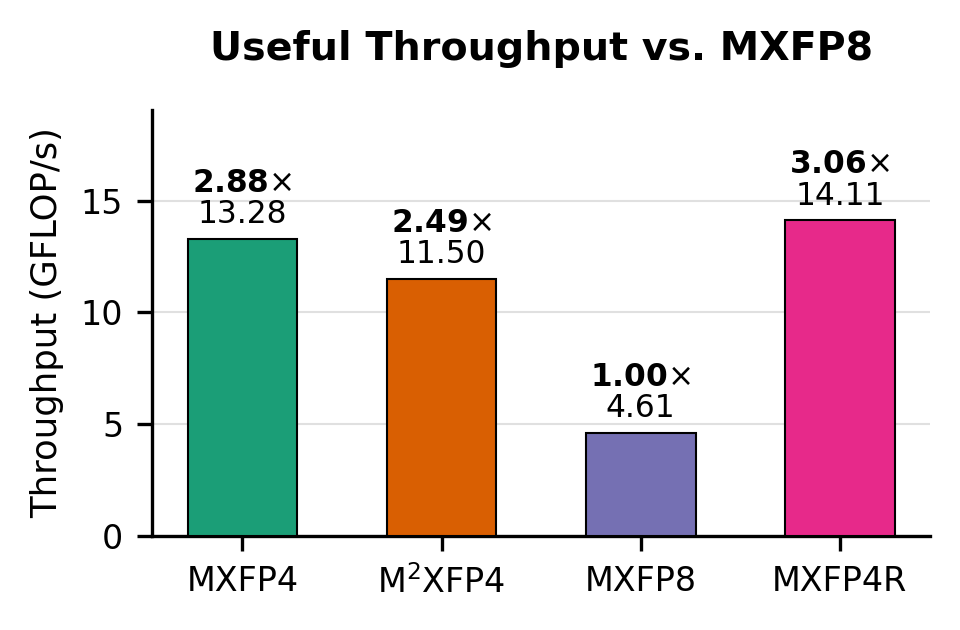
\includegraphics[width=\linewidth]{mxfp4r_throughput_comparison.png}
  \end{minipage}
\end{table*}

\section{Evaluation}
\label{sec:eval}

\subsection{Setup}
\label{sec:eval-setup}

Each engine is synthesised out of context with Yosys~\cite{wolf_yosys} through
the OpenROAD flow~\cite{ajayi2019openroad} at the Nangate45
\SI{45}{\nano\meter} node, under a common timing constraint.
Functional simulation uses Verilator~\cite{snyder_verilator}.

\subsection{Synthesis and throughput analysis}
\label{sec:eval-synthesis}

Physical synthesis results confirm our core hypothesis: specialising hardware datapaths to narrow microscaling formats yields significant area, frequency, and throughput density advantages over wider uniform representations.

First, our measurements demonstrate that narrow fused datapaths achieve superior physical efficiency. \fpfour{} emerges as the most compact and agile fused engine, requiring only \SI{13442}{\micro\meter\squared} and operating at \SI{414.9}{\mega\hertz}. This efficiency stems directly from its narrow four-bit multipliers and lightweight accumulation frame, compared to the 95-bit frame required by \fpeight. While \mtwo{} offers metadata refinements, its extra logic increases area and power consumption to \SI{441.0}{\milli\watt} while lowering maximum frequency to \SI{359.5}{\mega\hertz}. \fpeight{} requires the largest area (\SI{23881}{\micro\meter\squared}) and lowest frequency (\SI{288.3}{\mega\hertz}), confirming that wide uniform formats incur severe area and timing penalties that offset their element-level parallel gains.

Second, we establish that multi-instruction residue execution can overcome register file port constraints without sacrificing compute throughput. By decomposing the \fpfourres{} dot product into a decoupled instruction pair (\insn{mxr4dot} and \insn{mxfinal}), we eliminate the three-read-port register file bottleneck while unrolling combinational delay paths. The reduction stage (\insn{mxr4dot}) achieves \SI{915.5}{\mega\hertz}, and the accumulator stage (\insn{mxfinal}) reaches \SI{441.0}{\mega\hertz}. Sustaining one completed pair every two cycles yields a useful throughput of \SI{14.11}{\giga\flop\per\second}, representing a \SI{3.06}{\times} speedup over \fpeight{} (Fig.~\ref{fig:throughput_comparison}) and outperforming all single-instruction candidates.



\subsection{Unified evaluation framework}
\label{sec:eval-compare}

Because prior studies evaluated microscaling formats across different process nodes, synthesis flows, and host processors, published figures cannot be directly compared to isolate format-level trade-offs. To establish a rigorous benchmark, we reimplemented all format engines within a unified framework using the same RISC-V host core (\core), identical timing constraints, the open-source Yosys and OpenROAD toolchain, and the Nangate45 \SI{45}{\nano\meter} PDK.
\section{Conclusion}
\label{sec:conclusion}

This work evaluated \fpfourres, a residue MX format, by implementing it
alongside \fpfour, \fpeight, and \mtwo{} as format-specialised engines within a
single \xif-compliant coprocessor and characterising all four on a common core,
flow, and technology node. \fpfourres{} does not improve on \fpeight{} in
compute throughput, as its dual-scale dot product requires an instruction pair;
its benefit is a weight footprint equal to \fpfour{} at accuracy approaching
\fpeight, which favours memory-bound inference. The accompanying per-format
scale-free frame keeps each engine exact to round-to-nearest-even across the
full E8M0 scale range at a width set by its element format, and the coprocessor
is portable across \xif-compliant hosts.


\section*{Acknowledgment}
\ifanon
\else
  \TODO{Funding and institutional acknowledgments (camera-ready only).}
\fi
\emph{Use of AI.} The authors used AI tools to assist with (i) drafting portions of the manuscript text, (ii) generating figures, and (iii) writing RTL implementation code, all under the authors' direction. All AI-assisted output was reviewed, verified, and edited by the authors, who take full responsibility for the correctness and originality of the paper's content and results.


\balance
\bibliographystyle{IEEEtran}
\bibliography{references}

\end{document}